\newpage
\section{Credibility : robust evaluation methods}
%\begin{figure}[H]
%  \centering
%  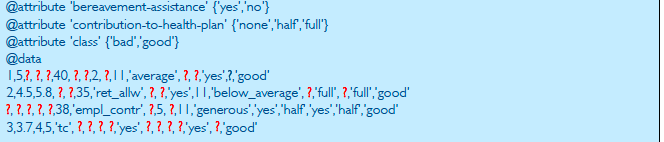
\includegraphics[width=.5\linewidth]{arffmissing}
%\end{figure}
When creating a model it is important to know :
\begin{enumerate}
\item how the model \textbf{performs}
\item how \textbf{reliable} the performance estimates are
\item how to \textbf{compare} performance of competing models
\item which model to choose if dealing with two equally performing models
\end{enumerate}

\subsection{Metric for performance evaluation}
\subsubsection{Regression}
\begin{itemize}
\item \textbf{Residual sum of squares}
$$ RSS(\overrightarrow{w}) = \sum \limits_{i=1}^{N} \left( y_i - \sum \limits_{j=0}^{D} w_jh_j(\overrightarrow{x_i}) \right)^2 $$
\item \textbf{Coefficient of determination}
$$ TSS = \sum \limits_{i=1}^{N}(y_i - \bar{y})^2$$
$$ R^2 = 1- \frac{RSS}{TSS}$$
$$ R^2_2 =  \frac{\sum \limits_{i=1}^{N}(\hat{y_i - \bar{y}})^2}{\sum \limits_{i=1}^{N}(y_i - \bar{y})^2}$$
\item \textbf{Mean square error}
$$ MSE= \frac{1}{N}\sum \limits_{i=1}^{N} (\hat{y_i}- y_i)^2$$
\item \textbf{Root mean square error}
$$ RMSE= \sqrt{\frac{1}{N}\sum \limits_{i=1}^{N} (\hat{y_i}- y_i)^2}$$
\end{itemize}
\subsubsection{Classification}
The \textbf{Confusion matrix} is a good way to evaluate classification tasks:
\begin{figure}[H]
  \centering
  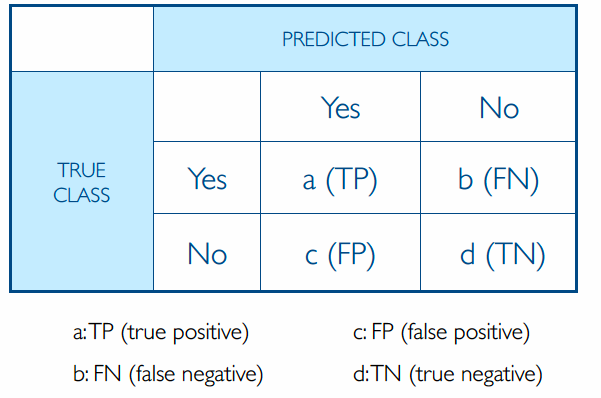
\includegraphics[width=.6\linewidth]{confmatrix}
\end{figure}

\begin{itemize}
\item  \textbf{Accuracy}
$$ \text{Accuracy} = \frac{TP + TN}{TP+TN+FP+FN}$$
How many right predictions over all the outcomes. \textbf{Not always a good choice} :  for example if 990/1000 example are class 0 and 10/1000 examples are class 1 predicting always class zero gives accuracy $99.9 \%$ which is useless since the interest is to predict class 1 (bank fraud example).
\item \textbf{Cost}
$$ C(x) = \text{ cost of missclassifying example of type x }$$
For example \textbf{FN} can be more "\textbf{expensive}" than \textbf{FP}:
\begin{figure}[H]
  \centering
  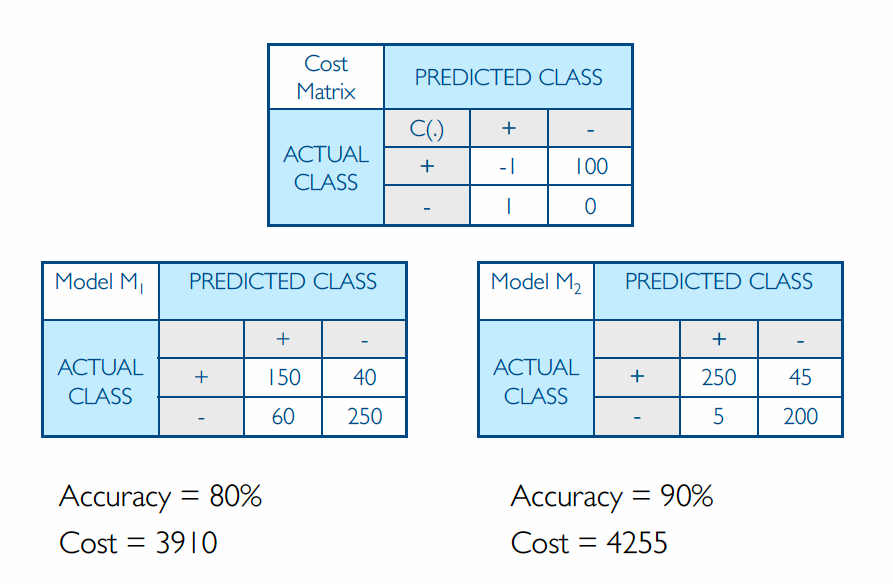
\includegraphics[width=.6\linewidth]{confmatrix2}
\end{figure}
This cost matrix can be used by some algorithms (like \textbf{Decision Trees}) to guide them.
\item \textbf{Precision}\\
Focuses on the percentage of examples that have been classified \textbf{positive} and \textbf{are actually positive}
$$ \frac{TP}{TP+FP}$$
higher precision = lower FP
\item \textbf{Recall}\\
Focuses on the percentage of examples that have been classified as positive with respect of the number of good existing examples 
$$ \frac{TP}{TP+FN}$$
higher recall = lower FN
\item \textbf{F1 measure}\\
Is biased towards all except \textbf{TN}
$$ \frac{2 \text{Recall} * \text{Precision}}{\text{Precision} + \text{Recall}}$$
\end{itemize}

\subsection{Methods for performance evaluation}
As already seen for regression and classification different methods can be used to evaluate a model (train/test split, CV...).
\begin{figure}[H]
  \centering
  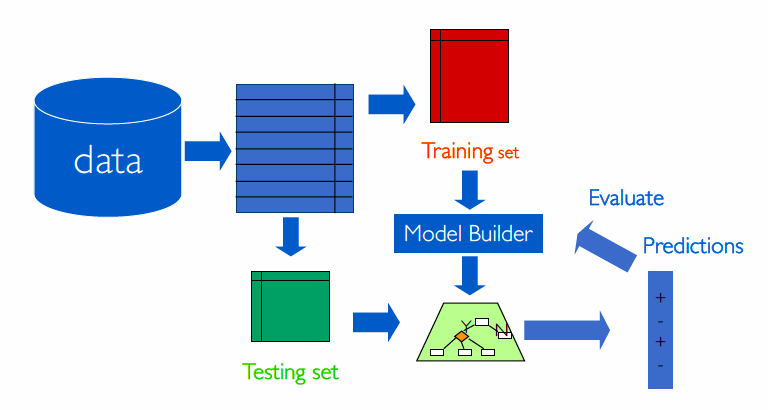
\includegraphics[width=.6\linewidth]{modeleval}
\end{figure}
It is important that \textbf{test data} is \textbf{never} used to train a model nor used to \textbf{tune parameters} :
\begin{itemize}
\item Train 
\item Test
\item Validation (used to tune parameters)
\end{itemize}
\begin{figure}[H]
  \centering
  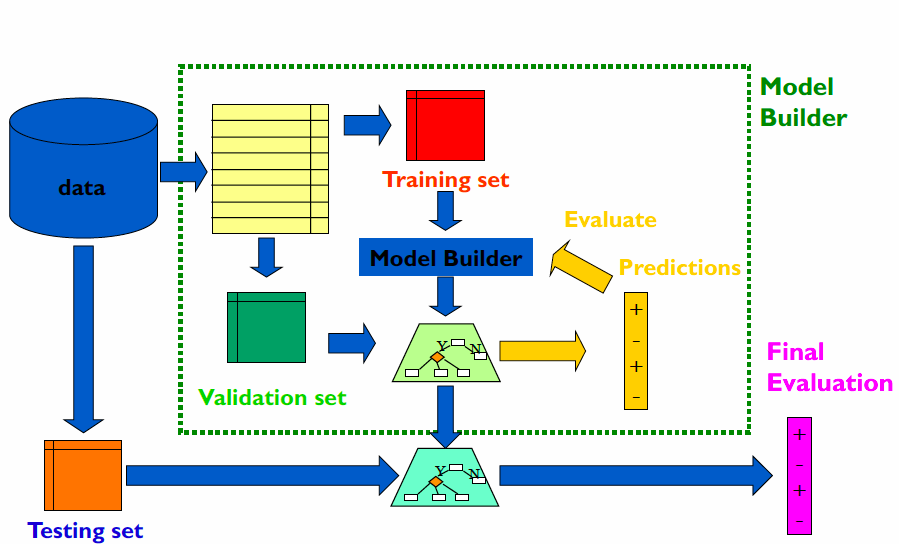
\includegraphics[width=.6\linewidth]{modeleval2}
\end{figure}
Performance of a model can depend on many factor (class distribution , cost of missclassfication , size of training and test sets ) and the estimated performance depends on the many methods :
\begin{itemize}

\item \textbf{Holdout}\\
Reserve $\frac{1}{3} \ \frac{2}{3}$ for training and $\frac{2}{3} \ \frac{1}{3}$ for testing. This method is \textbf{bad} for \textbf{small, unbalanced} as samples might not be representative ( it can produces training or test sets with only 1 class!).For this reason \textbf{stratified} sampling should be used : it makes sure that each class is represented \textbf{equally} in both subsets.
 
\item \textbf{Repeated holdout}\\
Holdout estimate can be made more reliable by \textbf{repeating} the process with \textbf{different} subsamples.In each iteration a certain proportion is \textbf{randomly selected} for training. The error rates are then \textbf{averaged} to yield an overall error rate.\\
The bad thing is that different test sets \textbf{overlap}

\item  \textbf{Cross validation}\\
\begin{enumerate}
\item Split data in k subsets of equal size
\item Each subset used in turn for testing while the rest for training.
\end{enumerate}
Better than repeated holdout because it does not overlap test sets. Even better performances are obtained by \textbf{shuffling} and \textbf{stratifying} (which reduces variance). Errors are again \textbf{averaged}.

\item \textbf{Leave-One-Out CV}\\
It is a particular form of CV that sets the number of fold = number of instances of training set. This makes best use of the data as only \textbf{one sample} is used for testing and the rest for training without using random sampling. The downside is that it is \textbf{computationally expensive} and does not allow \textbf{stratification}.

\item \textbf{Bootstraping}\\
Cross validation uses sampling without \textbf{replacement} :  the same instance, once selected , can not be selected again for a particular training/test set.
Bootstrap allows to \textbf{replace} samples :
\begin{itemize}
\item Sample a dataset of n instances with replacement to form a \textbf{new dataset} with n instances.
\item Use this dataset as \textbf{training set}
\item Use the instances that \textbf{don't occur in new training set} as \textbf{test set} (taken from original train set) 
An instance has probability  $1-\frac{1}{n}$ of \textbf{not} being picked , so ending up in the \textbf{test data} with probability :$$ \left( 1- \frac{1}{N} \right)^N \approx e^{-1} = 0.368$$ This means that the training data contain approximately $ 63.2 \% $ of the instances.\\
The \textbf{error estimate} will be very \textbf{pessimistic} since only $63.2\%$ of the data has been used. A good solution is to compute the \textbf{overall error} of training and testing : $$ \epsilon = 0.632 \cdot \epsilon_{test} + 0.368 \cdot \epsilon_{train}$$.
This process can be \textbf{repeated} with different replacement samples, averaging out the results.
\end{itemize}
\end{itemize}

\subsection{Compare competing models}
Suppose there are two models :
\begin{itemize}
\item Model $M_A$ with accuracy $82 \%$ using 10-fold CV
\item Model $M_B$ with accuracy $80 \%$ using 10-fold CV
\end{itemize}
How much \textbf{confidence} can we place on accuracy $M_A$ and $M_B$?
Is the statement $M_A$ is better than $M_B$ correct or can the difference be explained as "random fluctuations" in train/test set or even random luck?
To answer to this questions is to \textbf{measure the odds}:
\begin{itemize}
\item Apply \textbf{t-test}
\item Compute \textbf{p-value} (probability that the reported difference is due to chance)
\end{itemize}
An overall view of the possible combinations : 
\begin{figure}[H]
  \centering
  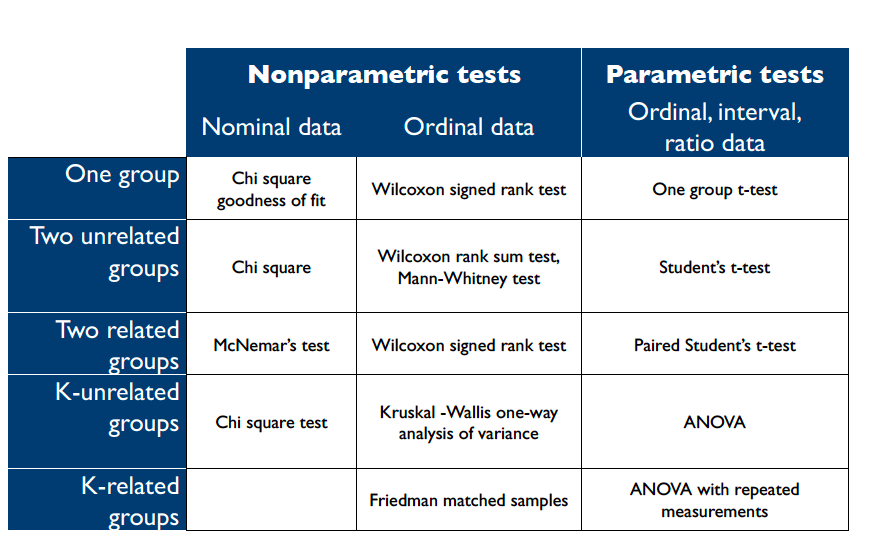
\includegraphics[width=.7\linewidth]{testcases}
\end{figure}

\subsubsection{Paired t-test using CV}
Generate \textbf{k-folds} and for each configuration compute the performances of Model A and Model B :
\begin{itemize}
\item $\theta^A_1 ... \theta^A_k$
\item $\theta^B_1 ... \theta^B_k$
\item $\delta_i = \theta^A_i - \theta^B_i$
\item $\mu_{\delta} =\frac{1}{k} \sum \limits_{i} \delta_i$ (mean)
\item $\sigma_{\delta} = \sqrt{\frac{1}{k} \sum \limits_{i}(\delta_i - \mu_{\delta})^2 }$ (stdev) 
\end{itemize}
The define the \textbf{two hypothesis}:
\begin{itemize}
\item $H_0 : \mu_{\delta} =0$
\item $H_1 : \mu_{\delta} \neq 0$
\end{itemize}
Then the \textbf{t-test} is applied to check whether the \textbf{null hypothesis} $H_0$ can be rejected with a \textbf{target confidence} :
\begin{figure}[H]
  \centering
  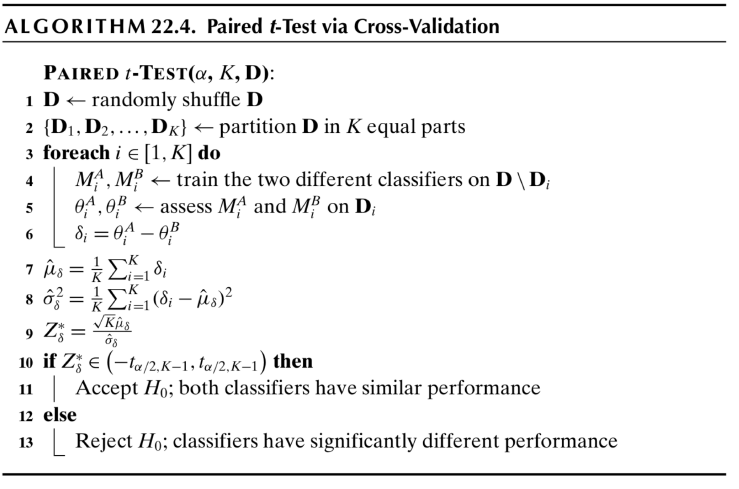
\includegraphics[width=.6\linewidth]{ttest}
\end{figure}
For example fixing the confidence at $95\%$ then the reported difference is statistically significant if the \textbf{p-value} is smaller than $1-c = 0.05$, otherwise if the \textbf{p-value } is \textbf{larger} than $0.05$ then the difference is \textbf{not } significant.\\
Note that the test can be done \textbf{paired} (estimates from \textbf{same} dataset) or \textbf{unpaired} (estimate from \textbf{differnet} datasets).


\subsubsection{Multiple testing}
Comparing performance of \textbf{several} classification algorithms requires a different approach . This is because :
\begin{itemize}
\item P(making a mistake) = $0.05$
\item P(not making a mistake) = $0.95$
\item P(making a mistake)$^{20}$  = $0.358$
\item P(not making a mistake)$^{20}$ = $0.642$
\end{itemize}
So when using 20 different methods there is a $64.2 \%$ chance of making at least one mistake.\\
Solutions:
\begin{itemize}

\item \textbf{Bonferroni Test}\\
Assumes that individual tests are independent.\\
Divides the threshold by the number of tests performed and \textbf{still use the t-test}:
\begin{itemize}
\item $\frac{0.05}{20} = 0.0025$
\item P(making a mistake) = 0.0025
\item P(making a mistake)$^{20}=0.0488$ 
\end{itemize}

\item \textbf{Non-Parametric tests}\\
A better way is to use non-parametric tests : they do not make any assumptions about the \textbf{distribution} of the variable population.\\
The two main tests are :
\begin{itemize}
\item \textbf{Mann-Whitney U Test} : non parametric equivalent of t-test
\item \textbf{Wilcoxon matched pairs singed rank test} : used to compare two related groups
\end{itemize}
\end{itemize}

\subsubsection{Probabilistic classifiers}
As already seen Logistic Regression is a classification method that used \textbf{probability} to predict labels $$ P(y_i|\overrightarrow{x_i})$$
So given an example $x_i$ it predicts a label with the \textbf{largest probability}, which is the equivalent of using a \textbf{threshold} of \textbf{0.5} :
$$ P(+1|x_i) = 0.55$$
$$ P(-1|x_i) = 0.45$$
$$ \text{Clearly the chosen class is +1 as it is} \geq 0.5$$
But \textbf{different thresholds} can be used : for example when we need a \textbf{bigger confidence} that the assigned label is 1 a threshold of 0.75 can be used.\\
Selecting a threshold \textbf{close to 1} (\textbf{pessimistic classifier}):
\begin{itemize}
\item \textbf{High precision }: not likely to produce \textbf{false positive} because the given threshold allows only very confident predictions to assign label 1.
\item \textbf{Low Recall}: there are likely many \textbf{false negatives}
\end{itemize}
Selecting a threshold \textbf{close to 0} (\textbf{optimistic classifier}):
\begin{itemize}
\item \textbf{Low Precision} : almost everything is positive
\item \textbf{High Recall} : minimum number of \textbf{false negatives}
\end{itemize}
Trade-off to \textbf{optimize} threshold!\\
\textbf{Precision-Recall curves} : 
\begin{figure}[H]
  \centering
  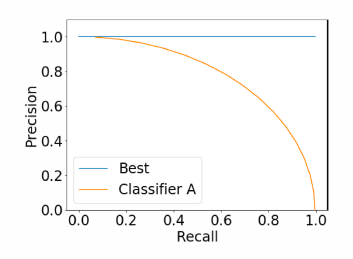
\includegraphics[width=.6\linewidth]{roccurve}
\end{figure}
Different classifiers show different shapes, to decide which is the best one:
\begin{itemize}
\item \textbf{Area under the curve} (closer to 1 = better)
\item \textbf{F1- Measure}
\end{itemize}

\subsubsection{ROC Curve}
Receiver operating	characteristic curve plots the \textbf{True positive} rate against the \textbf{False positive rate}
$$ TPR = \frac{TP}{TP+FN}$$
$$ FPR = \frac{FP}{FP+TN}$$
Each performance of a \textbf{classifier} is a \textbf{point} on the ROC curve. The location on the ROC curve of a classifier depends on :
\begin{itemize}
\item Threshold used for classification
\item Sample distribution
\item Cost matrix changes
\end{itemize}
The ideal situation is point \textbf{(0,1)} $\rightarrow$ \textbf{no} false positive , only \textbf{true positive}.
 \begin{figure}[H]
  \centering
  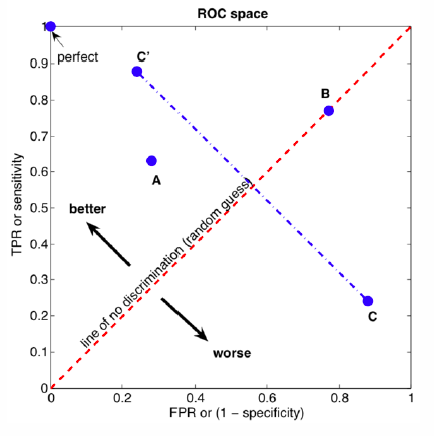
\includegraphics[width=.6\linewidth]{roccurve2}
\end{figure}
\begin{figure}[H]
  \centering
  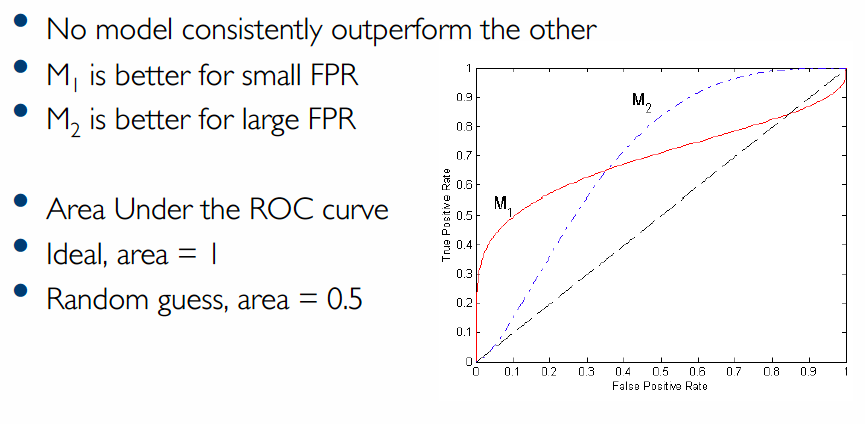
\includegraphics[width=.7\linewidth]{roccurve3}
\end{figure}

\subsection{Model Selection}
When building a model the trade-off between \textbf{model complexity} and \textbf{prediction accuracy} on training data is important : a good model must be \textbf{as simple} as possible but achieve high accuracy on the training data.
But finding the \textbf{best} algorithm is not always easy , as state by the \textbf{No Free Lunch Theorem}: if one algorithm \textbf{outperforms} another in a certain situation than it is due of its \textbf{fit to the particular problem} rather than the \textbf{superiority of the algorithm}. When dealing with a new problem it is important to gather information about \textbf{priori knowledge, data distribution,amount of data and cost/rewards.}	